% -*- mode: fundamental -*-

% ****************************************************************

\chapter{RISC-V: Functional verification of CPUs}

\markboth{Ch \arabic{chapter}: RISC-V: Verification}{\copyrightnotice}

\setcounter{page}{1}
% \renewcommand{\thepage}{\arabic{page}}
\renewcommand{\thepage}{\arabic{chapter}-\arabic{page}}

\label{ch_RISCV_verification}

% ****************************************************************

\section{Introduction}

\label{Sec_RISCV_verification_intro}

The last chapter described general techniques used to verify {\BSV}
designs of any kind.  This chapter focuses on techniques for
verification of CPU implementations.

Debugging and verifying a CPU implementation (whether it is a hardware
implementation or a software simulator) is hard because, as discussed
in Section~\ref{Sec_Interpreters}, it is not just a program, but is
itself an \emph{interpreter} of programs.  Thus we are confronted with
two levels, not one.  The first-level program (P1) is the CPU
implementation (the {\BSV} program), which we are simulating or running
in hardware.  P1, in turn, is interpreting the RISC-V program (P2)
that was loaded into the RISC-V CPU's memory. When we observe an error
in P2's outputs or behavior, it could be a bug in P2 (the RISC-V
program), or a bug in P1 (our RISC-V implementation), or both.

In other words, when we have an interpreter of programs, we
conceptually have an exponentially larger space of things to test
(test cases).  Every RISC-V program P2 is potentially a test case for
our implementation P1, along with every potential input to each P2!
This is illustrated in Figure~\ref{Fig_CPU_Verif_Complexity}.
\begin{figure}[htbp]
  \centerline{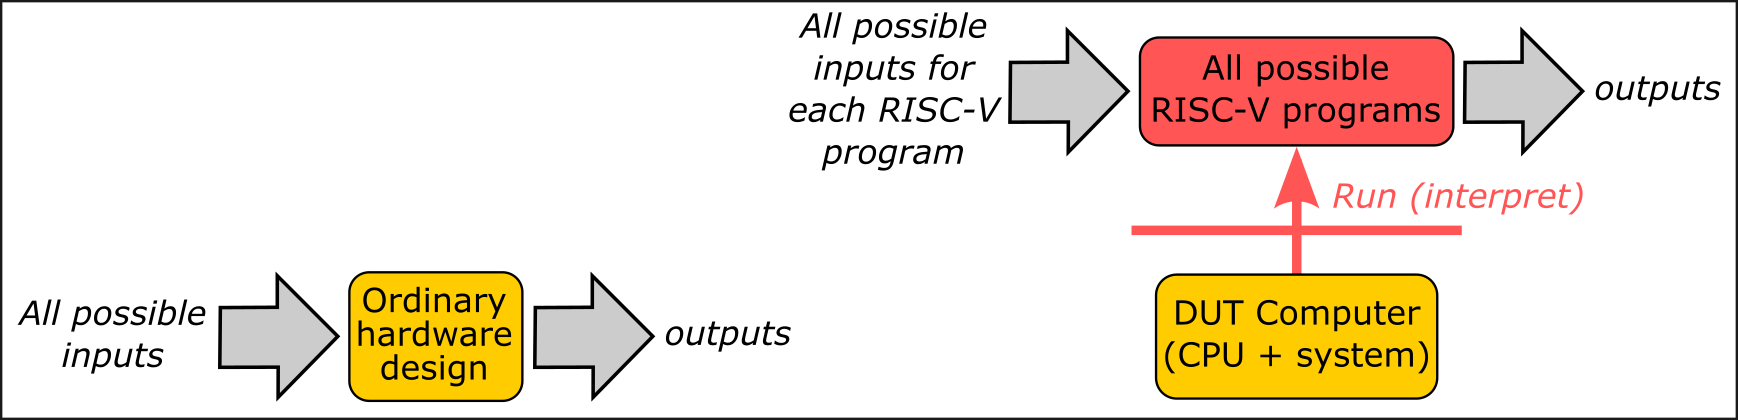
\includegraphics[width=6in,angle=0]{Figures/Fig_CPU_Verif_Complexity}}
  \caption{\label{Fig_CPU_Verif_Complexity}
           Complexity of CPU verification}
\end{figure}

In addition to this large space of potential tests, the duration of a
test can be very long.  A bug may exhibit itself only inside an
application program running under an operating system.  To reach this
point we may have to execute hundreds of millions, or billions of P2
instructions on P1.

Fortunately, for small to medium-sized isolated test programs, we can
exploit a key property the RISC-V ISA (and most ISAs): except for
interrupts, which are asynchronous events, and a few instructions
(such as \verb|rdtime| and \verb|rdcycle|, the sequence of
instructions executed by a RISC-V program on a particular initial
memory contents is completely deterministic and repeatable.  This
means that if we excute a RISC-V program P2 repeatedly in our test
setup, or even run P2 on different implementations (such as a software
simulator and Drum and Fife), they should all exhibit \emph{exactly}
the same sequence of instructions, or ``\emph{instruction trace}''.
If one of them takes a particular conditional BRANCH, then the others
should, as well.  If one of them traps due to, say, an illegal
instruction, then the others should, as well, and they all should
vector to exactly the same instruction address for the trap handler.
If one of them traps due to, say, an unimplemented memory location,
then the others should, too, assuming they have the same (or
equivalent) memory setup.  We call this a \emph{functional
equivalence} because different implementations perform the same
function on such a test program, even though they may execute it at
vastly different speeds.

Beyond small and medium-sized deterministic test programs, we need to
test the CPU in an environment that more closely resembles its
eventual operating environment.  This may include running operating
systems and interacting with devices that may generate timer and
device interrupts asynchronously, {\ie} at unpredictable moments in
time relative to instruction execution.  This topic is discussed in
Section~\ref{Sec_Asymmetric_Tandem_Verification}.

This chapter only addresses the question of \emph{functional
correctness} (``Does the CPU compute correct data?'').  An equally
important topic is \emph{performance correctness} (``Does the CPU
compute results in the allowed/expected time?'').  That topic is
addressed in Chapter~\ref{ch_Optimization}.

% ****************************************************************

\section{Trusted functional simulators (``golden reference models'')}

\index[RV]{Trusted functional simulator}
\index[RV]{Simulator!trusted, functional}
\index[RV]{Golden Reference Model}

Most CPU design teams rely on a ``trusted'' software functional
simulator that can execute RISC-V programs.  Such a simulator is
written, and is maintained, with a focus that prioritizes clarity and
correctness, not speed.  This simulator acts as a reference standard,
and is also called a ``Golden Reference Model''.  It answers questions
such as:

\begin{itemize}
 \item What is a correct execution when executing a RISC-V program P2?

 \item What is the correct architectural state (registers, CSRs, memory) before
     and after each instruction I$_j$?

\end{itemize}

We can compare our hardware implementation against this reference to
see if our hardware implementation is also behaving correctly.

Often, a trusted simulator is the first thing one implements when
designing a new ISA, before starting any hardware design.  Once the
ISA is frozen, because the functional simulator is only defining
functional correctness (not speed), it can be used across multiple
hardware CPU design projects, {\ie} it is a long-lived resource that
can be shared across multiple projects.

For the RISC-V ISA, there are several free and open-source software
functional simulators available that we can use as a trusted
reference.  Appendix~\ref{apx_resources_trusted_simulators} provides
URL links to the two most well-known, the \emph{Spike} simulator and
the \emph{Sail} simulator.  Each of them can be configured for a
particular subset of the RISC-V ISA (such as RV32IM, or RV64IMAFDC,
with or without privilege levels and virtual memory, {\etc}), and then
run RISC-V programs, producing a log/trace of the instructions
executed.

It can be useful to be able to modify and customize a trusted software
functional simulator.  For example, if we are extending the RISC-V ISA
with new, custom instructions, then we would like the simulator to
support them.  Or, we may want extra information detail in the
simulator's output trace that was not originally provided.
Or, we may use the simulator in non-standard ways, such
as the asymmetric tandem verification mode described in
Section~\ref{Sec_Asymmetric_Tandem_Verification}.

Being open-source, the Spike and Sail simulators can be modified for
custom purposes.  Many companies also have their own trusted software
RISC-V functional simulators for greater modifiability and
customization (such as \emph{Cissr} from Bluespec, Inc.).

Golden reference models are usually written as RISC-V interpreters in
a software programming language (for example, Spike is written in
C++).  In this case they only run as software on a standard computer.

Golden reference models can also be written in a high-level hardware
design language, such as {\BSV}.  For example, we can think of Drum in
this way.  Because it is a simple FSM, it is extremely simple and
clear.  The advantage of a hardware golden reference model is that it
can be synthesized into hardware and plugged into any system
environment where a more powerful CPU implementation will be go.

% ****************************************************************

\section{RISC-V test programs for verification}

\label{Sec_test_suites}

An advantage of an open (non-proprietary) ISA like RISC-V is that
there is a vast and growing worldwide community of hardware CPU
developers---companies, universities, research organizations, students
and hobbyists---who share a common need for RISC-V test programs for
verification.  Many of the test programs they create are shared in
free and open-source form.

% ================================================================

\subsection{ISA tests}

The oldest and most stable set of test programs originated the the
University of California Berkeley with the original RISC-V team, and
is now maintained and expanded by RISC-V International (RVI) on their
GitHub site at
\url{https://github.com/riscv-software-src/riscv-tests}.  These are a
set of several hundred test programs written in RISC-V Assembly
Language.  Each program contains a small set of tests for some
particular instruction in the RISC-V ISA.  The tests cover RV32I and
RV64I and the A, M, F, D and C extensions; machine, supervisor and
user extensions; and some system features like PMP (Physical Memory
Protection).  Most user-level tests can be built to run with or
without virtual memory.  The tests are provided in source-code form
(RISC-V Assembly Language) and need to be compiled with a C compiler
({\eg} \emph{gcc}) to produce ELF binaries.

The tests are small (a few thousand instructions) and are all
\emph{self-checking}, {\ie} they compute something and then check if
the result has the expected value.  At the end of the test, each
program outputs a PASS/FAIL indicator.  PASS means it passed all the
tests in the file. In the FAIL case, it also outputs the test number
within the file that failed.

The tests are small enough that it is feasible manually to compare a
trace from our CPU implementation against the assembly-language source
code (or the assembly language in the \emph{gcc}-produced ``objdump''
disassembly of the ELF file) and analyze it for errors.

The tests also run sufficiently quickly (a few minutes at most) that
we routinely and automatically rerun all the ISA tests every time we
make any significant change to the CPU design's source code or test
environment.

% ================================================================

\subsection{ACTs and other test suites}

RVI (RISC-V International) is developing a set of tests called ACTs
(Architecture Compatibility Tests).  Each test is a RISC-V program
that runs and produces a final ``signature'', which is a reliable hash
of the final state (PC, registers, CSRs, memory, {\etc}).

If a candidate RISC-V CPU implementation claims to support, say,
RV32IM, then it must run the relevant ACTs for RV32IM, and the
produced signatures should match the official signature for that test
published by RVI (the official signatures, in turn, are produced by
RVI by running on a trusted simulator such as Spike or Sail).

This is an ongoing project. Some relevant links:

\begin{tabbing}
\hmm \= \url{https://wiki.riscv.org/pages/viewpage.action?pageId=49872986} \\
     \> \url{https://github.com/riscv-non-isa/riscv-arch-test} \\
     \> \url{https://riscof.readthedocs.io/en/stable/}
\end{tabbing}

Another test suite, called ``riscv-dv'', was developed initially at
Google; subsequent stewardship was taken over by the ChipsAlliance
non-profit group.  These tests generate ``random'' RISC-V programs
(constrained to a certain ISA subset), run the program on a candidate
implementation which should generate a trace, and compare against a
trace from a trusted functional simulator:

\begin{tabbing}
\hmm \= \url{https://github.com/chipsalliance/riscv-dv}
\end{tabbing}

In addition, most organizations maintain their own collection of test
programs and ``regression suites'' (programs that previously surfaced
a bug in some implementation, which are continuously re-run to ensure
that the bug has not resurfaced due to more recent changes).

% ================================================================

\subsection{What does ``verified'' mean? Levels of assurance and coverage}

\index[RV]{Formal verification}
\index[BSV]{Formal verification}

\begin{figure}[htbp]
  \centerline{\includegraphics[width=0.8\textwidth,angle=0]{Figures/Fig_Levels_of_Assurance}}
  \caption{\label{Fig_Levels_of_Assurance}
           Levels of Assurance}
\end{figure}

In the software community, the term ``verified program'' has
historically meant ``formally verified program'', {\ie} that we have a
\emph{proof of correctness} of the program against a formal
specification of the program.  A formal specification is usually
written in a specialized formal specification language which are
usually highly mathematical, declarative languages.  A formal proof of
correctness uses formal tools (theorem provers, mechanized logics) to
show that a candidate implementation correctly computes something
prescribed by the formal spec.  Formal verification may not involve
executing the implementation at all, just analysis of the code for the
implementation.  Formal verification may be partial (prove that the
implementation is correct for certain inputs) or complete (for all
inputs).  Although there has been huge progress in formal verifcation
over the decades, as of 2024 it is still not able to handle very large
and complex programs; it is used very successfully for individual or
small collections of modules, and for partial correctness.

The hardware community has also been exploring formal verifation of
hardware implementations, and there are several tools offered
commercially.  But, as in in the software community, as of 2024 it is
still not able to handle very large and complex designs; it is used
quite successfully for individual or small collections of modules, and
for partial correctness.

In the hardware community, the term ``verification'' has historically
meant ``extensive testing with a large suite of test programs'', not
formal verification.  One can think of the term ``level of assurance''
as a point on scale ranging from ``no assurance'' (untested, unproved)
to ``full assurance'' (formally proved correct).
Figure~\ref{Fig_Levels_of_Assurance} illustrates the relationship of
formal and traditional hardware verification.

As we increase the number and variety of test programs that we run
(the test suite), we may increase the level of assurance that we have
a correctly implemented design.  In the rare and unlikely case that
the set of inputs is small enough that we can test all of them, we
essentially have full assurance, or a proof of correctness by
enumeration.  Normally, the space of possible tests is too large even
to enumerate, let alone run.  Thus the test suite needs to be
carefully engineered and selected to \emph{cover} as much of the space
as feasible, particularly the space of inputs expected when the design
is deployed in the field.

The term ``coverage'' is a kind of measure of level of assurance.  It
can be used both in a functional way (``How much of the space of
possible inputs has been tested?'') or in a more
implementation-specific way (``What fraction of the lines of code in
the {\BSV}/Veri\-log/System\-Veri\-log source have we exercised with
our tests?'').

% ================================================================

\subsection{Testing regimes}

Here is a sequence of testing regimes with increasing simulation times
but also increasing levels of assurance of the correctness of our CPU
implementation:

\begin{itemize}
 \item Run all the standard ``ISA tests'' mentioned in Section~\ref{Sec_test_suites}.

 \item Run the ACTs and riscv-dv test suites mentioned in Section~\ref{Sec_test_suites}.

 \item Run a small operating system (such as FreeRTOS or Zephyr).
       This will check correct handling of timer interrupts, and
       possibly memory maps and physical memory protection (PMPs).

 \item Run the kernel of a full-service operating systsem (such as the Linux kernel).

 \item Run a standard distribution a full-service operating systsem
       (such as Debian Linux or Ubuntu Linux), {\ie} the OS kernel
       \emph{plus} the pre-load of all the applications and service
       programs that come with distribution (including block devices
       and networking).

\end{itemize}

The latter items are often executed on FPGA because simulation speed may be too slow.

% ****************************************************************

\section{A testbench for Drum and Fife}

Figure~\ref{Fig_CPU_Simulation} illustrates the structure of the
testbench provided with this book for Drum and Fife.
\begin{figure}[htbp]
  \centerline{\includegraphics[width=6in,angle=0]{Figures/Fig_CPU_Simulation}}
  \caption{\label{Fig_CPU_Simulation}
           Top-level simulation setup for the Drum and Fife CPUs}
\end{figure}
On the left we see the top-level of the module hierarchy, and on the
right we see some module interactions.  The top-level module,
\verb|mkTop|, has the \verb|Empty| interface.

The interface for Drum and Fife, \verb|CPU_IFC|, was described in
Section~\ref{Sec_Drum_CPU_interface}.  The most important
sub-interfaces are the FIFOs carrying IMem and DMem memory requests
and responses.  \verb|mkTop| instantiates the \verb|mkCPU| module
(which can be either Drum or Fife) and \verb|mkMems_Devices| modules.
An excerpt from \verb|mkTop| is shown below:

\SHOWCODE{Code_Extracts/mkTop.tex}

Note that we pass the CPU's IMem and DMem sub-interfaces directly to
Mems\_Devices module as module parameters; as a result, rules in
\verb|mkMems_Devices| can directly access the IMem and DMem FIFO
interfaces of the CPU to collect IMem and DMem requests and send back
IMem and DMem responses.

The \verb|mkMems_Devices| module implements models for memory, a UART
(Universal Asynchronous Receiver/Transmitter, also known as a serial
port), a real-time clock, and any other devices expected by the CPU
and the RISC-V code running on the CPU.  Some of these (memory, UART,
Fife store-buffer) are implemented by importing C code.

The memory system in the testbench also needs a way to be pre-loaded
with the binary RISC-V code of the program that we want the CPU to
execute, before the CPU begins executing.

A rule in \verb|mkTop| that fires at the beginning of simulation
invokes the methods \verb|cpu.init| and \verb|mems_devices.init|,
passing them a struct with some initialization parameters, such as the
reset value for the PC (address from which the first instruction will
be fetched), and a file descriptor into which logs should be written.

\SHOWCODE{Code_Extracts/Top_init.tex}

Another rule in \verb|mkTop| fires on every clock.  On each clock, it
retrieves a value reprsenting the wall-clock time from
\verb|mems_devices| and relays it into the CPU:

\SHOWCODE{Code_Extracts/Top_relay_time.tex}

Other than that, \verb|mkTop| plays no further role in execution.
Rules inside \verb|mkCPU| operate the CPU, putting out IMem and DMem
requests.  Rules inside \verb|mkMems_Devices| operate the memory and
device models, returning IMem and DMem responses.

We do not intend to describe \verb|mkMems_Devices| in any more detail
here, since it is outside the main focus of this book, the Drum and
Fife CPUs.  Section~\ref{Sec_Importing_C} has details on how to import
C code into {\BSV}.  The interested student is welcome to peruse the code
in the \verb|src_Top/| directory.

% ****************************************************************

\section{Symmetric Tandem Verification of CPU implementations}

\label{Sec_Symmetric_Tandem_Verification}

\index[RV]{Tandem verification!symmetric}

In Section~\ref{Sec_RISCV_verification_intro} we mentioned that the
instruction trace for a RISC-V program is mostly deterministic and
repeatable across RISC-V implementations.  We can exploit this
property in a setup called \emph{symmetric tandem verification},
illustrated in Figure~\ref{Fig_tandem_verification}.
\begin{figure}[htbp]
  \centerline{\includegraphics[width=0.6\textwidth,angle=0]{Figures/Fig_tandem_verification}}
  \caption{\label{Fig_tandem_verification}
                  Symmetric Tandem Verification}
\end{figure}

We load the same ELF RISC-V binary file into the memories of a
``trusted'' simuator and our DUT (Design Under Test) setup, and have
them both run the program.  We arrange to have both simulators write
out a trace of their respective program executions.  Then, we compare
the two traces. Any difference in the traces is an indicator of a
potential bug in the DUT.

For example, we might find that, at a certain conditional BRANCH
instruction in P2, the trusted simulator took the branch whereas our
implementation did not.  This would indicate either that there is some
problem with our implementation of the conditional BRANCH instruction,
or that there was a problem in some previous instruction that computed
one or both of the register values used by the conditional BRANCH
instruction.  Thus, debugging is a process of identifying exactly
which instruction in our implementation ``went wrong'', {\ie} did
something different from what the trusted simulator did.

% ================================================================

\subsection{Configuration}

The trusted simulator and the DUT setup the should be configured
``identically'':

\begin{itemize}
 \item They should support the same RISC-V ISA subset, so that an
       illegal instruction in one is also an illegal instruction in the
       other.  

 \item They should have the same (or equivalent) memory systems, so
       that an illegal or misaligned memory access in one has the same
       response in the other.

 \item They do not need to have the same \emph{temporal} behavior.
       For example, memory access latency in one need not match memory
       latency in the other, and the ``time'' taken to execute any
       particular instruction in one need not match the ``time'' taken
       by the other.

\end{itemize}

% ================================================================

\subsection{Level of detail in traces}

Traces can be produced at varying levels of detail.  For example, for
each instruction executed, we could record:

\begin{tightlist}
 \item just the PC;
 \item or also the instruction iself;
 \item or also any values it reads from or writes to registers
\end{tightlist}

More detail means more simulation overhead (slower simulation) to
produce the trace.  Traces can become very large ({\eg} gigabytes when
tracing, say, the booting of an OS).  But more detail can also provide
better ``resolution'' in identifying the location of a bug.  For
example, suppose one instruction (I1) computes a wrong value and
stores it to memory, where it sits for thousands, perhaps millions of
instructions before it is loaded into a register (instruction I2) and,
some instructions later, this is used in a conditional BRANCH
instruction (instruction I3).  The wrong value may cause the trusted
simulator and the DUT to diverge, where one takes the branch, the
other does not, which we detect because the next PCs are different.
If our trace only records PCs, then we will detect a difference only
at I3. However if we also record register values, we will detect the
difference earlier, at I1 or I2.

One way to reduce excessive detail is to record traces only for a
certain window of instructions, say starting at the 10 millionth
instruction and for the following one thousand instructions.  This
would be fine if we were guaranteed that there was no divergence until
the 10 millionth instruction, but we have no way of knowing that.  A
way to address this is:

\begin{itemize}

 \item Run the trusted simulator withoug producing any trace until 10M
       instructions, and record a ``snapshot'' of \emph{the entire
       architectural state}---PC, all registers, CSRs, all of memory.
       Then, continue for 1K instructions, producing a trusted trace.

 \item Initialize the DUT's PC, registers and memory with the values
       in the snapshot, and then let the DUT execute for 1K
       instructions, producing a DUT trace to compare with the trusted
       trace.

\end{itemize}

This requires infrastructure support in the trusted simulator to be
able to dump a snapshot, and in the testbench to be able to initialize
its state using the snapshot.

% ================================================================

\subsection{Online {\vs} offline tandem verification}

The setup in Figure~\ref{Fig_tandem_verification} can be performed
offline or online:

\begin{itemize}

 \item {\bf Offline}: Each of the two simulators records its trace in
       a file, and these files are compared later, manually, or with
       ``{\tt diff}'', or with a specialized comparison tool.  In
       fact, for a given test program, the reference simulator need be
       run only once, and its trace can be saved for future
       comparisons.

 \item {\bf Online}: The two simulators are run concurrently ({\eg}
       two processes in an operating sytem).  They each generate their
       trace into a \emph{stream} such as an operating system ``pipe''
       or ``tty'' or network connection.  A comparison tool runs
       concurrently as a third process, continually consuming the two
       trace streams and comparing them immediately.

\end{itemize}

The online setup requires more infrastructure and tooling, but has
some advantages.  First, it can abort both simulations as soon as it
detects a divergence, so we don't unnecessarily continue simulating
for a long time.  Second, since the compare tool is continually
consuming the traces, it need not be recorded in a file, thereby
eliminating the ``trace-file size'' problem.

% ****************************************************************

\section{Asymmetric tandem verification and ``full-system'' verification}

\label{Sec_Asymmetric_Tandem_Verification}

We said in Section~\ref{Sec_Symmetric_Tandem_Verification} that,
except for interrupts (asynchronous events), the two traces (from the
trusted simulator and the DUT) should be identical.  There are some
nuances to this claim.

% ================================================================

\subsection{Instructions with non-deterministic results}

If a RISC-V program uses the \verb|rdcycle| or \verb|rdtime|
instructions, then the results, loaded into registers, will likely be
different in the two setups.

% ================================================================

\subsection{Reading uninitialized memory}

If the memories in the trusted simulator and the DUT setup have not
been initialized identically, then a LOAD instruction can return
different results in the two setups, even in ``bug-free'' RISC-V
programs.  For example, when traversing a C string (one character per
byte), the program may only LOAD aligned 8-byte doublewords, for more
efficiency. At the end of the string, only a prefix of the 8 loaded
bytes may be part of the string, and the remaining bytes may be
``uninitialized'' or random.  The C program may correctly examine only
those bytes that are in the string.  However, a tandem verifier will
not be aware of this, and may compare the full 8 bytes loaded by the
trusted simulator and the DUT, and falsely identify a difference
because bytes outside the string happen to be different.

% ================================================================

\subsection{Devices and interrupts}

Simulating the DUT may require running code that interacts with
devices or device models because they are fundamental to the CPU's
intended applications.  Thus, the DUT simulation needs to model more
of the ``full system'' in which it is intended to be used.  Devices or
device models may be unique or proprietary to the intended application
domain.  Devices contain memory-mapped locations accessed by the
RISC-V program, and may generate interrupts.  We cannot expect the
trusted simulator (which is often created and maintained by others) to
model all these devices.

% ================================================================

\subsection{Asymmetric mode}

All the above issues can be handled if we take an ``asymmetric'' view
of tandem verifaction, and if we can configure the trusted simulator
to work in ``tandem verification mode''.  This is illustrated in
Figure~\ref{Fig_tandem_verification_II}.
\begin{figure}[htbp]
  \centerline{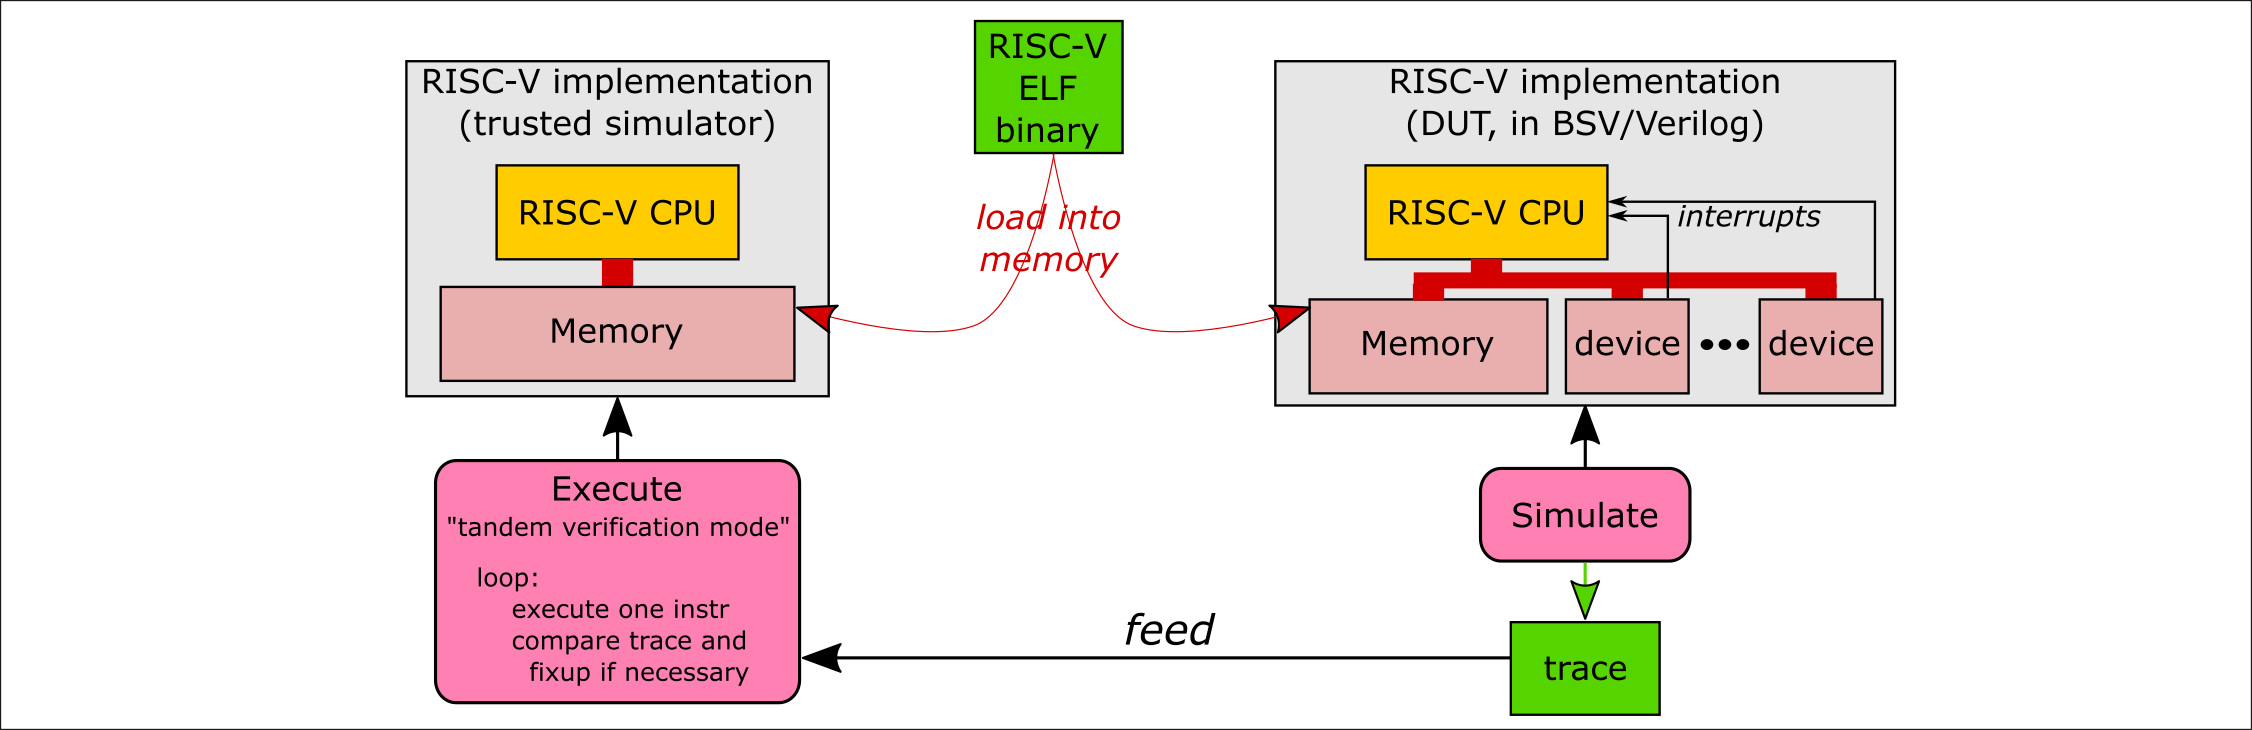
\includegraphics[width=0.7\textwidth,angle=0]
                              {Figures/Fig_tandem_verification_II}}
  \caption{\label{Fig_tandem_verification_II}
           Asymmetric tandem verification: dealing with ``minor'' differences,
           interrupts (asynchronous events), devices, {\etc}}
\end{figure}

Here, the DUT simulation produces a CPU execution trace, including a
record of the interrupts received and taken.  This trace is fed to the
trusted simulator which runs in tandem verification mode.  In this
mode, before simulating each instruction, it examines the next ITEM in
the trace, and:

\begin{itemize}

 \item If ITEM is an interrupt received (bit set in the DUT CPU's CSR
       MIP), then also set that bit in the trusted simulator's CSR
       MIP.  This brings the trusted simulator's CSR back ``in sync''
       with the DUT, from where we proceed.

 \item If ITEM is an interrupt taken: check if the trusted simulator
       can also take this same interrupt at this time (correctly set
       interrupt bits in CSR MIP, correctly set interrupt-enable bits
       in CSRs MIE, MSTATUS {\etc}).  If so, then perform the
       interrupt-taking actions in the trusted simulator (save values
       in CSRs \verb|mepc|, \verb|mcause| and \verb|mtval|, update CSR
       \verb|MSTATUS|, set the PC to the value in CSR \verb|mtvec|,
       {\etc}).  If this interrupt cannot be taken here, report a
       divergence and stop.

 \item Otherwise (ITEM is an instruction-execution), perform the next
       instruction in the trusted simulator and compare results with
       ITEM.

       If the instruction is a LOAD, RDTIME or RDCYCLE and the loaded
       values are different, report the difference, but do not stop,
       do a ``fixup'' and continue:

       \begin{tightlist}

	\item Update the loaded value in the trusted simulator to be
              the same as in the DUT trace.  This brings the trusted
              simulator's registers back ``in sync'' with the DUT,
              from where we proceed.

       \end{tightlist}

\end{itemize}

In summary: the trusted simulator need not model any devices at all,
just memory.  Instead of generating a trace, it checks the
DUT-produced trace for correctness.

% ****************************************************************

\section{Tandem verification with real hardware (FPGA or ASIC)}

The discussion above on Tandem Verification assumed that the trusted
model and the DUT were both being run in simulation.  But, of course,
there is nothing simulation-specific about the technique.

If the RISC-V CPU \emph{hardware} is capable of generating traces, and
the infrastructure supports streaming that trace out of the hardware
to a host machine then, once again, the trace can be compared with
that of a trusted simulator.

The trusted model can itself be written in a synthesizable hardware
description language like {\BSV}.  In fact, the Drum CPU could be a
candidate, because it is an extremely simple implementation, not
designed for speed, and so possibly trustworthy.  In this case, the
entire setup in Figure~\ref{Fig_tandem_verification_II} could be in
hardware, which is likely to run several orders of magnitude faster
than any simulation.

% ****************************************************************
